\section{Introduction}\label{sec:positioningIntroduction}
The sensors which were used in a autonomous vehicle are very important for the final result.
If the sensors are worse the whole vehicle never can bring a good result.
But not only the sensor is important for the behavior of the car.
Also software which read out the value and filter and correct them is very important.

This chapter will present some sensors which can be used to get information about the environment of the car.
During this chapter different sensors, interfaces, bugs are explained.
The next step is to create categories to rate the different sensors.
Another part of this chapter is to calculate the most possible current position based on the input data of different sensors.

First the main categories and sensors which are aviable are listed:
\begin{itemize}
\item Absolute Sensors
	\subitem Lateration
		\subsubitem GPS	
		\subsubitem Mobile telephony
	\subsubitem Gyro
\item Environment Detection
	\subitem Image Recognition
	\subitem Bumper Sensor
	\subitem Distance Sensor
		\subsubitem Ultrasonic
		\subsubitem Infrared
	\subitem Floor Sensor
\item Relative Sensors
	\subitem Touch less
		\subsubitem Acceleration
		\subsubitem Magnetometer
	\subitem Inertia
		\subsubitem Rotary Encoder
		\subsubitem Mouse Sensor
\end{itemize}


\section{Criteria for Kind of Sensors}
To rate the sensors a lot of criteria have to be considered.


\subsection{Measures Fails, Tolerance, Errors}
\begin{figure}
\makebox[\linewidth]{
%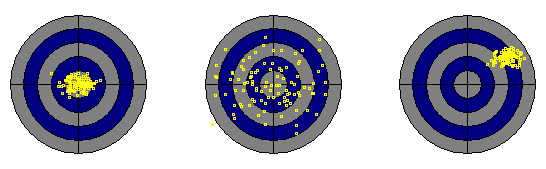
\includegraphics[scale=0.5]{picturesPositioning/precisionDarts.png}
%Draw dart
\pgfmathsetmacro{\drawSize}{0.65}

\newcommand*{\drawDart}[2]{
	\providelength{\dartCurrentSize}
	\setlength{\dartCurrentSize}{#1}
	\provideboolean{dartColor}
	\setboolean{dartColor}{true}
	\whiledo {\dartCurrentSize > 0}
	{
		\ifdartColor
			\path[fill=blue,draw=black] (0,0) circle (\dartCurrentSize);
		\else
			\path[fill=gray,draw=black] (0,0) circle (\dartCurrentSize);
		\fi
		\addtolength{\dartCurrentSize}{-#2}
		\setboolean{dartColor}{\ifdartColor false\else true\fi}
	}
 }

\newcommand*{\calcRealPos}[1]{
	\FPmul\pos{#1}{\drawSize}
}

\newcommand*{\drawFixDart}{
	\calcRealPos{3}
	\FPmul\partSize{\pos}{0.10}
	\drawDart{\pos cm}{\partSize cm}
}

\newcommand{\calcRandCirclePos}{
	\loop
		\pgfmathsetmacro{\posx}{rand}
		\pgfmathsetmacro{\posy}{rand}
		\FPmul\squarex{\posx}{\posx}
		\FPmul\squarey{\posy}{\posy}
		\FPadd\squaresum{\squarex}{\squarey}
		\ifdim \squaresum pt > 1pt
	\repeat
}

\newcommand{\drawPoint}[2]{
	\calcRealPos{#1}
	\pgfmathsetmacro{\posx}{\pos}
	\calcRealPos{#2}
	\path[draw=yellow] (\posx cm,\pos cm) circle (0.1cm);
}

\begin{tikzpicture}
\drawFixDart
\providecounter{ct}
\pgfmathsetseed{1}
\forloop{ct}{0}{\value{ct} < 30}{
	\calcRandCirclePos
	\FPmul\posx{\posx}{0.5}
	\FPmul\posy{\posy}{0.5}
	\drawPoint{\posx}{\posy}
}
\end{tikzpicture}

\begin{tikzpicture}
\drawFixDart
\providecounter{ct}
\forloop{ct}{0}{\value{ct} < 70}{
	\calcRandCirclePos
	\FPmul\posx{\posx}{2}
	\FPmul\posy{\posy}{2}
	\drawPoint{\posx}{\posy}
}
\end{tikzpicture}

\begin{tikzpicture}
\drawFixDart
\providecounter{ct}
\forloop{ct}{0}{\value{ct} < 70}{
	\calcRandCirclePos
	\FPmul\posx{\posx}{0.5}
	\FPadd\posx{\posx}{1}
	\FPmul\posy{\posy}{0.5}
	\FPadd\posy{\posy}{0.7}
	\drawPoint{\posx}{\posy}
}
\end{tikzpicture}

\begin{tikzpicture}
\drawFixDart
\providecounter{ct}
\forloop{ct}{0}{\value{ct} < 70}{
	\calcRandCirclePos
	\FPmul\posx{\posx}{0.5}
	\FPmul\posy{\posy}{0.5}
	\drawPoint{\posx}{\posy}
}
\drawPoint{2}{2}
\calcRealPos{3.1} \pgfmathsetmacro{\posfromx}{\pos}
\calcRealPos{3.1} \pgfmathsetmacro{\posfromy}{\pos}
\calcRealPos{2.1} \pgfmathsetmacro{\postox}{\pos}
\calcRealPos{2.1} \pgfmathsetmacro{\postoy}{\pos}
\draw[->, line width=2pt,color=red] (\posfromx,\posfromy) -- (\postox,\postoy);
\drawPoint{-1}{2.5}
\calcRealPos{-2.1} \pgfmathsetmacro{\posfromx}{\pos}
\calcRealPos{3.6} \pgfmathsetmacro{\posfromy}{\pos}
\calcRealPos{-1.1} \pgfmathsetmacro{\postox}{\pos}
\calcRealPos{2.6} \pgfmathsetmacro{\postoy}{\pos}
\draw[->, line width=2pt,color=red] (\posfromx,\posfromy) -- (\postox,\postoy);
\end{tikzpicture}
}
\caption{Error Types}%\cite{img:precisionDarts}}
\label{fig:errorTypes}
\end{figure}
The used sensors have different properties.
One is faster and the another one have a higher precision.
In this section the different types of errors which a sensor can produce are explained.


\subsubsection{Methodical Errors}
Methodical errors are errors which are expectable.
This means the errors have similar properties.
They occurs mainly when devices are badly calibrated.
A example of a methodical error is the right picture of Errors~\ref{fig:errorTypes}.
This example shows that methodical errors are those which are the easiest one to create an algorithm which calculates the real value.
Such a algorithm could be also a simple addition or multiplication.
Also a calibration of the device can help to improve the result.


\subsubsection{Run Away Values}
Run away values are single measure results which doesn't fit in the expected range.
This means that most of the values which are measured are close to the real value except a very small count of values.
A very popular example for a run away value are the red pixels in a photo which was made by a digital camera.
Although the most pixel fit very well there are some pixel which return a value which is to much red.
This effect of digital cameras come through when the image sensor get to hot.
However, this effect that heat increase the error rate is not only by image sensors.
Also other sensors produce much more errors if they become hot.
The type of error which is produced through heat can be very different.
Some sensors lose precision other produce a methodical error.
Often sensors produce combined bugs.


\subsubsection{Brake Down}
A break down is when a sensor lose its full functionally.
The way a brake down can be recogniced could be very different.
The worsest thing which could happen is when device produce a shortbrake because this can also damage the whole car.
This scenario is realy rare.
Most times the device will return a constant value like zero or the digital interface can't be acces any more.
In such a case the software shouldn't hang up.
In a intelligent autonoumas software the car should recognice that the sensor will not react any more and it should stop asking and waiting for the answer.
Instead of the broken sensor the software should chose another sensor which is perhaps not as good as the old one but bether than nothing.


\subsubsection{Bad Precision}
This type of error is that one which is much heavier to handle than other errors.
In case of a bad precission the sensor doesn't return the value as precission as required.
So the returned value can be seen as random number in a defined range of the real value
A possibility to handle this error is to calculate the average value of some meassures.
This method has the disadvantage that short high or low values of the real input dissapears.


\subsection{Output Value Format}
The different types of sensors requires different ways a sensor can return its value.
Mainly the return type can be categorized in analog and digital values.
But this is a very vague grouping because some sensors return values which contain properties of analog and digital values as well.
On the other hand there are sensors which offer their results in two or more interfaces and so they are analog and digital sensors at the same time.


\subsubsection{Analog}
The most cheap sensors are analog sensors.
This sensors are most the cheaper one because they don't need any logic to interpret the result.
In most cases the sensors have a internal logic to filter and optimize the result.
The group of analog sensors can be split up in sensors which return a current and sensors where its resistor can be measured.


\paragraph{Voltage Source}
Sensors which return a analog voltage have the problem that the returned voltage and also the returned current is very small.
Examples for analog sensors which return a voltage are:
\begin{itemize}
\item Photo Diode
\item pH Sensor
\item Peltier Element
\end{itemize}
The photo diode produces a very small amount of energy when a photon with sufficient energy hits the junction layer of a diode.
This is called the photoelectric effect.
So a photo diode work like a very small solar pane.
Another sensors which return a current is a pH sensor or a peltier element where the seeback effect is used.
And so a big amount of analog sensors return a very small voltage with a very small maximal current.
To measure the result the returned voltage or the returned current have to be amplified.
For example it is possible to amplify the current of a photodiode with a transistor and add a pull-up resitor to the collector of the resitor.
Then the voltage between the resitor and the transistor which is in relation to the amplified current can be measured.
For an illustatrion see figure~\ref{fig:phototransistorWithPullUp}.


\begin{figure}
\center
\begin{circuitikz}
\draw(0,0)
	to[american voltage source] (0,2)
	to[R] (2,2)
	to[leD*] (2,0)
	-- (0,0);
\draw (5,1) node[npn] (trans) {}
	(trans.base) node[anchor=east] {}
	(trans.collector) node[anchor=south] {}
	(trans.emitter) node[anchor=north] {};
\draw(3,0)
	to[pDo,mirror](3,2)
	--(5,2)
	--(trans.collector);
\draw(5,2)
	--(5,2)
	to[R,*-o](5,4) node[above]{V};
\draw(5,2)
	to[short,*-o](6,2) node[right]{ADC};
\draw(trans.emitter)
	to[short,-o](5,0) node[below]{GND};
\draw (3,0)
	--(3.5,0)
	--(3.5,1)
	--(trans.base);
\end{circuitikz}
\caption{Phototransistor with pull up resistor}
\medskip
\small
This circuit layout shows a photo-transistor which is connected to to the microcontroller and a pull-up resistor.
\label{fig:phototransistorWithPullUp}
\end{figure}



\paragraph{Resistor}
A lot of sensors return the result as a resistor value.
Examples for such sensors are:
\begin{itemize}
\item Air Humidity
\item Pressure
\item Bight
\item Expansion
\item Lightness
\item Photo-transistor
\item ...
\end{itemize}
To measure the value of a resistor different circuits can be used.
The well known methods are:
\begin{itemize}
\item Voltage Divider
\item Wheatstone Bridge
\item ...
\end{itemize}
The voltage divider has the advantage that it has a very simple structure.
The result of the measurement is a voltage which can be read directly by a microcontroller's DAC.
The disadvantage of the voltage divider is, that it is not as exact as the wheatstone bridge.
The Wheatstone bridge has a very high precision but it is more difficult to use and build.


\subsubsection{Binary}
A lot of sensors return a binary signal which means that only a logical high and a logical low is allowed.
All values between are not allowed.
The most binary sensors are analog sensors which have a constant threshold.
To convert a analog signal to a binary signal a schmitt-trigger can be used.
Example for such sensors are:
\begin{itemize}
\item Distance
\subitem Floor Existence
\item Enough Power Supply Voltage
\item Light Barrier
\item Rotary Encoder Detector 
\end{itemize}


\subsubsection{Digital}
A lot of sensors use a digital interface to transmit the measured value.
Such sensors have the advantage, that the result need not to be converted by the microcontroller's analog digital converter.
This has the advantage, that the analog input pin can be used for other things.
Although the microcontroller's analog digital converter have a big scale range it is not as good because of the precision.
The problem of the those converter is that they have a random noise.
Examples for digital interfaces which were used by sensors are:
\begin{itemize}
\item I2C
\item UART
\item ...
\end{itemize}


\subsubsection{Quadrature Output}
\begin{figure}
\makebox[\linewidth]{

\includegraphics[height=0.2 \textheight]{picturesPositioning/rotaryEncoderPatternQuadrature.jpg}
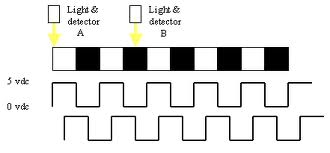
\includegraphics[height=0.2 \textheight]{picturesPositioning/quadratureOutput.jpg}
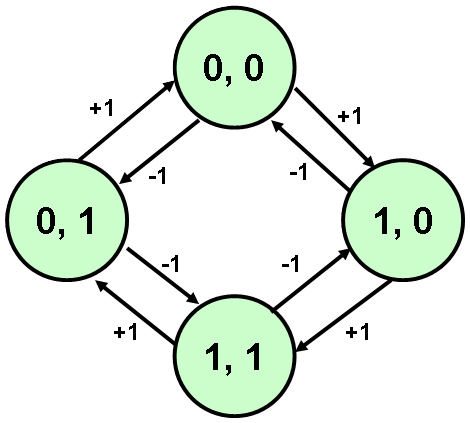
\includegraphics[height=0.2 \textheight]{picturesPositioning/quadratureStates.jpg}


}
\caption{Pattern of a quadrature rotary encoder, the output and the states}
\label{fig:quadratureRotaryEncoder}
\end{figure}

A quadrature output is a signal which is transmitted with two binary wires.
On each wire a square wave is transmitted.
This two scare waves overlaps and so the precision is doubled.
This two wires can have 4 states:
\begin{itemize}
\item Low, Low
\item Low, High
\item High, Low
\item High, High
\end{itemize}
The big advantage of this system is that also the direction can be calculated.
The simplest way to find out the direction is to compare the high of the other wire at a phase change.
An illustration of this is figure~\ref{fig:quadratureRotaryEncoder}.
The measured value is the sum of all in- and decrements.
Examples for sensors which uses the quadrature output are:
\begin{itemize}
\item Rotary Encoder
\item Mouse Sensor
\item ...
\end{itemize}


\section{Selection}
A very important step to create a system which can calculate its own position is the selection of sensors.
At least the different types of categories have to be rated.
This table~\ref{tab:categoryRating} should illustrate this.
This table is made up by the rating categories and the different sensors groups.
Both rating significance and sensor group rating is a value between and inclusive zero and ten.
The rated value describes the positive property of the current category.
As example:\\
\begin{tabular}{l|l|l}
& 0 & 10 \\
Methodical Error & Many & None\\
Amount of Software & 100 code lines & 1-2 code lines\\
Computing Load & 1\% of the available capacities & 50 of the available capacities\\
\end{tabular}
The chosen sensor category rating should be a average representative value for the sum of all different sensors in this group.
If there exist sensor which can be connected with I2C and sensors which can be connected with DAC's then the halve of the points which would be subtracted from I2C are subtract. The same rating algorithm is applied to DAC's.



\newcommand*{\ratingSignificance}[1]{
\providecounter{ratingLine} %ratingline = the rating of the category
\providecounter{ratingPartSum}
\providecounter{ratingFinalSum}
\setcounter{ratingLine}{#1}#1
\addtocounter{ratingPartSum}{#1}
\addtocounter{ratingFinalSum}{#1}
}

\newcommand*{\ratingPartialSum}{
\arabic{ratingPartSum}
\setcounter{ratingPartSum}{0}
}

\newcommand*{\ratingFinalSum}{
\arabic{ratingFinalSum}
\setcounter{ratingFinalSum}{0}
}

\newcommand*{\rating}[2]{
\providecounter{ratingSave#1} %ratingSave<name> = the category-rating of the sensor
\setcounter{ratingSave#1}{#2}#2
}

%ratingMultiplied = the absolut category rating of the sensor
%ratingSaveResult = the summarized absolut category ratings of the sensor
%ratingFinalSaveResult<name> = the final result
\newcommand*{\ratingResult}[1]{\providecounter{ratingMultiplied}\providecounter{ratingPartialResult#1}\providecounter{ratingFinalResult#1} \setcounter{ratingMultiplied}{\value{ratingSave#1} * \value{ratingLine}}\addtocounter{ratingPartialResult#1}{\value{ratingMultiplied}}\addtocounter{ratingFinalResult#1}{\value{ratingMultiplied}}\arabic{ratingMultiplied}}

\newcommand*{\ratingPartialResult}[1]{\arabic{ratingPartialResult#1}\setcounter{ratingPartialResult#1}{0}}

\newcommand*{\ratingFinalResult}[1]{\arabic{ratingFinalResult#1}\setcounter{ratingFinalResult#1}{0}}

\newcommand*{\sensorRatingSum}{
\cline{2-25}
& Sum & \ratingPartialSum  & &
\ratingPartialResult{acc} & &
\ratingPartialResult{bum} & &
\ratingPartialResult{gps} & &
\ratingPartialResult{gyr} & &
\ratingPartialResult{idi} & &
\ratingPartialResult{ifl} & &
\ratingPartialResult{ire} & &
\ratingPartialResult{mag} & &
\ratingPartialResult{mou} & &
\ratingPartialResult{rot} & &
\ratingPartialResult{udi} \\
}
\newcommand*{\sensorFinalSum}{
\hline
\multicolumn{2}{|l|}{Sum} & \ratingFinalSum &  &
\ratingFinalResult{acc} &  &
\ratingFinalResult{bum} &  &
\ratingFinalResult{gps} &  &
\ratingFinalResult{gyr} &  &
\ratingFinalResult{idi} &  &
\ratingFinalResult{ifl} &  &
\ratingFinalResult{ire} &  &
\ratingFinalResult{mag} &  &
\ratingFinalResult{mou} &  &
\ratingFinalResult{rot} &  &
\ratingFinalResult{udi}\\
\hline
}

\begin{sidewaystable}

\makebox[\linewidth]{
\begin{tabular}{|l|l|l||c|c|c|c|c|c|c|c|c|c|c|c|c|c|c|c|c|c|c|c|c|c|}
\cline{1-2}
\multicolumn{2}{|l|}{Category} &  
\leaningLabelB{Significance} &
\multicolumn{2}{c}{\leaningLabel{Accelometer} }&
\multicolumn{2}{c}{\leaningLabel{Bumper Sensor} } & 
\multicolumn{2}{c}{\leaningLabel{GPS} } &
\multicolumn{2}{c}{\leaningLabel{Gyro} } &
\multicolumn{2}{c}{\leaningLabel{Infrared Distance Sensor} } &
\multicolumn{2}{c}{\leaningLabel{Infrared Floor Sensor} } &
\multicolumn{2}{c}{\leaningLabel{Image Recognition} } &
\multicolumn{2}{c}{\leaningLabel{Magnetometer} } &
\multicolumn{2}{c}{\leaningLabel{Mouse Sensor} } &
\multicolumn{2}{c}{\leaningLabel{Rotary Encoder} } &
\multicolumn{2}{c}{\leaningLabel{Ultrasonic Distance Sensor} } \\
\hline
\multirow{3}{*}{  \rotatebox{90}{ Bugs~ } }
& Methodical Error & \ratingSignificance{2} & 
\rating{acc}{6} & \ratingResult{acc} & 
\rating{bum}{10} & \ratingResult{bum} &
\rating{gps}{5} & \ratingResult{gps} &
\rating{gyr}{6} & \ratingResult{gyr} &
\rating{idi}{7} & \ratingResult{idi} &
\rating{ifl}{10} & \ratingResult{ifl} &
\rating{ire}{4} & \ratingResult{ire} &
\rating{mag}{6} & \ratingResult{mag} &
\rating{mou}{8} & \ratingResult{mou} &
\rating{rot}{8} & \ratingResult{rot} & %e.a.: Different wheel start position
\rating{udi}{7} & \ratingResult{udi} \\

& Run Away Value & \ratingSignificance{2} &
\rating{acc}{6} & \ratingResult{acc} & 
\rating{bum}{10} & \ratingResult{bum} &
\rating{gps}{5} & \ratingResult{gps} &
\rating{gyr}{6} & \ratingResult{gyr} &
\rating{idi}{6} & \ratingResult{idi} &
\rating{ifl}{10} & \ratingResult{ifl} & 
\rating{ire}{4} & \ratingResult{ire} &
\rating{mag}{6} & \ratingResult{mag} &
\rating{mou}{9} & \ratingResult{mou} &
\rating{rot}{10} & \ratingResult{rot} &
\rating{udi}{6} & \ratingResult{udi} \\

& Brake Down Possibility & \ratingSignificance{1} &
\rating{acc}{9} & \ratingResult{acc} & 
\rating{bum}{2} & \ratingResult{bum} & %Parts with high mechanical stress
\rating{gps}{5} & \ratingResult{gps} & %Inside a house
\rating{gyr}{9} & \ratingResult{gyr} &
\rating{idi}{8} & \ratingResult{idi} & %Light pollution
\rating{ifl}{8} & \ratingResult{ifl} & %Black line on floor
\rating{ire}{9} & \ratingResult{ire} &
\rating{mag}{9} & \ratingResult{mag} &
\rating{mou}{9} & \ratingResult{mou} &
\rating{rot}{9} & \ratingResult{rot} &
\rating{udi}{9} & \ratingResult{udi} \\

& Precision & \ratingSignificance{4} &
\rating{acc}{5} & \ratingResult{acc} & 
\rating{bum}{10} & \ratingResult{bum} &
\rating{gps}{0} & \ratingResult{gps} & 
\rating{gyr}{5} & \ratingResult{gyr} &
\rating{idi}{8} & \ratingResult{idi} &
\rating{ifl}{10} & \ratingResult{ifl} &
\rating{ire}{4} & \ratingResult{ire} &
\rating{mag}{6} & \ratingResult{mag} &
\rating{mou}{9} & \ratingResult{mou} &
\rating{rot}{9} & \ratingResult{rot} &
\rating{udi}{8} & \ratingResult{udi} \\

\sensorRatingSum
\hline
\multirow{3}{*}{ \rotatebox{90}{ Usability } }
& Amount of Software &  \ratingSignificance{1} &
\rating{acc}{8} & \ratingResult{acc} & 
\rating{bum}{9} & \ratingResult{bum} &
\rating{gps}{2} & \ratingResult{gps} & 
\rating{gyr}{8} & \ratingResult{gyr} &
\rating{idi}{5} & \ratingResult{idi} &
\rating{ifl}{9} & \ratingResult{ifl} &
\rating{ire}{0} & \ratingResult{ire} &
\rating{mag}{8} & \ratingResult{mag} &
\rating{mou}{2} & \ratingResult{mou} &
\rating{rot}{8} & \ratingResult{rot} &
\rating{udi}{5} & \ratingResult{udi} \\

& Amount of Algorithms &  \ratingSignificance{1} &
\rating{acc}{10} & \ratingResult{acc} & 
\rating{bum}{10} & \ratingResult{bum} &
\rating{gps}{2} & \ratingResult{gps} & 
\rating{gyr}{10} & \ratingResult{gyr} &
\rating{idi}{3} & \ratingResult{idi} &
\rating{ifl}{10} & \ratingResult{ifl} &
\rating{ire}{0} & \ratingResult{ire} &
\rating{mag}{10} & \ratingResult{mag} &
\rating{mou}{8} & \ratingResult{mou} &
\rating{rot}{9} & \ratingResult{rot} &
\rating{udi}{3} & \ratingResult{udi} \\

& Amount of Hardware &  \ratingSignificance{1} &
\rating{acc}{9} & \ratingResult{acc} & 
\rating{bum}{8} & \ratingResult{bum} & %Schmitt-Trigger
\rating{gps}{7} & \ratingResult{gps} & 
\rating{gyr}{9} & \ratingResult{gyr} &
\rating{idi}{7} & \ratingResult{idi} &
\rating{ifl}{7} & \ratingResult{ifl} &
\rating{ire}{7} & \ratingResult{ire} &
\rating{mag}{9} & \ratingResult{mag} &
\rating{mou}{5} & \ratingResult{mou} &
\rating{rot}{5} & \ratingResult{rot} &
\rating{udi}{8} & \ratingResult{udi} \\
\sensorRatingSum

\hline
\multirow{3}{*}{ \rotatebox{90}{ Resources~ } }
& Computing Load & \ratingSignificance{7} &
\rating{acc}{8} & \ratingResult{acc} & 
\rating{bum}{10} & \ratingResult{bum} &
\rating{gps}{2} & \ratingResult{gps} & 
\rating{gyr}{8} & \ratingResult{gyr} &
\rating{idi}{6} & \ratingResult{idi} &
\rating{ifl}{10} & \ratingResult{ifl} &
\rating{ire}{0} & \ratingResult{ire} &
\rating{mag}{8} & \ratingResult{mag} &
\rating{mou}{6} & \ratingResult{mou} &
\rating{rot}{8} & \ratingResult{rot} &
\rating{udi}{6} & \ratingResult{udi} \\

& Interrupt Pins & \ratingSignificance{2} &
\rating{acc}{10} & \ratingResult{acc} & 
\rating{bum}{5} & \ratingResult{bum} & % 1 * 50%
\rating{gps}{10} & \ratingResult{gps} & 
\rating{gyr}{10} & \ratingResult{gyr} &
\rating{idi}{10} & \ratingResult{idi} &
\rating{ifl}{5} & \ratingResult{ifl} & % 1 * 50%
\rating{ire}{10} & \ratingResult{ire} &
\rating{mag}{10} & \ratingResult{mag} &
\rating{mou}{2} & \ratingResult{mou} & % 2 * 40%
\rating{rot}{0} & \ratingResult{rot} & % 4 * 100% -- 1*100%
\rating{udi}{10} & \ratingResult{udi} \\

& DAC Pins & \ratingSignificance{1} &
\rating{acc}{4} & \ratingResult{acc} & % 3
\rating{bum}{10} & \ratingResult{bum} & % 0
\rating{gps}{10} & \ratingResult{gps} & % 0
\rating{gyr}{4} & \ratingResult{gyr} & % 3
\rating{idi}{6} & \ratingResult{idi} &% 1
\rating{ifl}{8} & \ratingResult{ifl} & % 0
\rating{ire}{9} & \ratingResult{ire} & % 0 - x
\rating{mag}{4} & \ratingResult{mag} & % 3
\rating{mou}{10} & \ratingResult{mou} & % 0
\rating{rot}{10} & \ratingResult{rot} & % 0
\rating{udi}{8} & \ratingResult{udi} \\ % 1

& Digital Pins & \ratingSignificance{1} &
\rating{acc}{10} & \ratingResult{acc} & % 0
\rating{bum}{8} & \ratingResult{bum} & % 1
\rating{gps}{0} & \ratingResult{gps} & % 4 -- 10
\rating{gyr}{4} & \ratingResult{gyr} & % 0
\rating{idi}{10} & \ratingResult{idi} & % 0
\rating{ifl}{8} & \ratingResult{ifl} & % 1
\rating{ire}{0} & \ratingResult{ire} & % ~7
\rating{mag}{10} & \ratingResult{mag} & % 0
\rating{mou}{3} & \ratingResult{mou} & % 2 -- 4
\rating{rot}{4} & \ratingResult{rot} & % 2 --4
\rating{udi}{6} & \ratingResult{udi} \\ % 1

& PWM Pins & \ratingSignificance{1} &
\rating{acc}{10} & \ratingResult{acc} & % 0
\rating{bum}{10} & \ratingResult{bum} & % 0
\rating{gps}{10} & \ratingResult{gps} & % 0
\rating{gyr}{10} & \ratingResult{gyr} & % 0
\rating{idi}{10} & \ratingResult{idi} & % 0
\rating{ifl}{10} & \ratingResult{ifl} & % 0
\rating{ire}{10} & \ratingResult{ire} & % 0
\rating{mag}{10} & \ratingResult{mag} & % 0
\rating{mou}{10} & \ratingResult{mou} & % 0
\rating{rot}{10} & \ratingResult{rot} & % 0
\rating{udi}{10} & \ratingResult{udi} \\ % 0

& I2C Address & \ratingSignificance{1} &
\rating{acc}{5} & \ratingResult{acc} & % 1
\rating{bum}{10} & \ratingResult{bum} & % 0
\rating{gps}{5} & \ratingResult{gps} & % 1
\rating{gyr}{5} & \ratingResult{gyr} & % 1
\rating{idi}{10} & \ratingResult{idi} & % 0
\rating{ifl}{10} & \ratingResult{ifl} & % 0
\rating{ire}{5} & \ratingResult{ire} & % 1
\rating{mag}{5} & \ratingResult{mag} & % 1
\rating{mou}{5} & \ratingResult{mou} & % 1
\rating{rot}{10} & \ratingResult{rot} & % 0
\rating{udi}{5} & \ratingResult{udi} \\ % 1

& UART Port & \ratingSignificance{1} &
\rating{acc}{10} & \ratingResult{acc} & % 0
\rating{bum}{10} & \ratingResult{bum} & % 0
\rating{gps}{10} & \ratingResult{gps} & % 0
\rating{gyr}{10} & \ratingResult{gyr} & % 0
\rating{idi}{10} & \ratingResult{idi} & % 0
\rating{ifl}{10} & \ratingResult{ifl} & % 0
\rating{ire}{10} & \ratingResult{ire} & % 0
\rating{mag}{10} & \ratingResult{mag} & % 0
\rating{mou}{10} & \ratingResult{mou} & % 0
\rating{rot}{10} & \ratingResult{rot} & % 0
\rating{udi}{10} & \ratingResult{udi} \\ % 0
\sensorRatingSum
\sensorFinalSum
\end{tabular}
}
\caption{The categories with the specific rating}
\label{tab:categoryRating}
\end{sidewaystable}



The important part of this selection is both the kind and the type of sensor which is used.
There are different criteria which are typical for the kind of sensor.
First the criteria are shown and then the different kind of sensors are rated.


\section{$\cancel{Combine Different Sensors}$}